The aim of this literature review is to provide a comprehensive understanding of the key concepts and technologies that underpin this project.

These include microservices architecture and front-end development using Flutter. This review will serve as the theoretical foundation for the design and implementation of a microservices-based e-commerce application for a souvenir e-shop, along with a front-end application using Flutter.
In the next section, we will delve deeper into microservices architecture, starting with its definition and core principles.
\section{Microservices Architecture}
\subsection{Overview of Microservices Architecture}
Microservices architecture is a design approach where an application is built as a collection of small services. Each of these services runs in its own process and communicates with others using lightweight mechanisms, often an HTTP resource API. These services are built around business capabilities and are independently deployable by fully automated deployment machinery.
\begin{figure}[H]
    \centering
    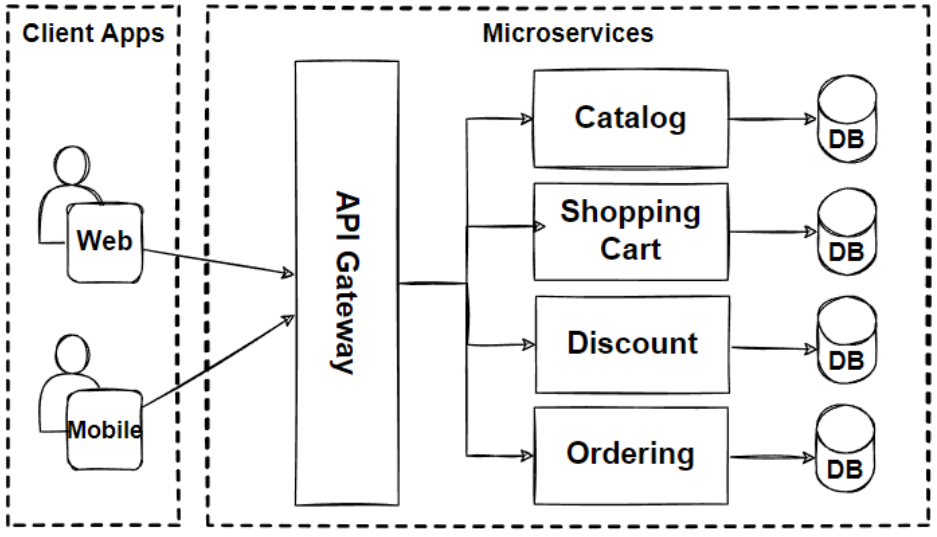
\includegraphics[width=.64\linewidth]{../images/micoservices_visualization.png}
    \caption{Microservices}\label{Fig:NN}
\end{figure}

For instance, consider an e-commerce application. In a monolithic architecture, all functionalities like user management, product catalog, order processing, and payment system would be in a single codebase. In contrast, in a microservices architecture, each of these functionalities would be a separate service with its own database and business logic.

\subsection{Benefits of Microservices:}
The benefits of using microservices architecture in e-commerce applications are numerous. They include improved scalability as each service can be scaled independently based on demand, increased resilience as the failure of a single service does not affect the entire system, and enhanced agility and speed in bringing new features to market.

\textbf{Amazon} is a prime example of the benefits of microservices. Originally, Amazon had a monolithic architecture, but as their services expanded, they moved to a microservices architecture. This allowed them to scale individual services based on demand. For example, during a sale, the order processing service could be scaled up without affecting other services.

\subsection{Challenges of Microservices:}

Despite its benefits, microservices architecture presents several challenges:
\begin{itemize}
    \item[-] \textbf{Complexity:} Managing multiple services can be complex, requiring sophisticated coordination and orchestration.
    \item[-] \textbf{Distributed Data Management:} Handling distributed data across services can be difficult and requires careful consistency management.
    \item[-] \textbf{Communication Overhead:} Implementing communication between services can introduce additional latency and resource usage.
\end{itemize}

\textbf{Netflix} faced challenges with microservices when they first transitioned from a monolithic architecture. They had to deal with complexities in managing multiple services and ensuring data consistency across services. They also faced challenges in implementing communication between services.

\section{Microservices in ASP.NET}
In this project, a new souvenir e-shop will be implemented using a microservices architecture from the ground up with ASP.NET. Each feature such as product management, inventory management, order processing, and payment processing will be implemented as a separate microservice running in its own Docker container.
\subsection{ASP.NET and Microservices}
ASP.NET is a robust framework for .NET that simplifies the creation of APIs, which form the backbone of microservices. It provides built-in support for Docker containers, which are lightweight and can be easily managed, making them ideal for deploying microservices.

ASP.NET offers high performance, which is critical in a microservices architecture where each service should be highly responsive. The high throughput of .NET surpasses many popular frameworks, making it an excellent choice for building efficient microservices.
\subsection{Communication Between Services}
In a microservices architecture built with ASP.NET, secure communication between services is crucial. Technologies like HTTPS provide secure communication over a computer network, while RabbitMQ with MassTransit in ASP.NET offers a reliable and efficient message broker system, which is essential for communication between microservices.

\subsection{Docker and .NET Tools}
Docker has become a standard in the container industry due to its ability to encapsulate microservices in containers, enhancing their isolation, portability, and scalability. .NET is built to work seamlessly with Docker, allowing developers to focus on building their microservices without worrying about compatibility issues.

The Visual Studio family of products offers comprehensive tools for developing ASP.NET applications with Docker support on Windows.
These tools simplify the process of configuring applications for Docker and allow developers to step through their code line-by-line as it runs in a Docker container.
\section{Introduction to Flutter and Clean Architecture}
\subsection{Flutter}
Flutter is an open-source UI software development kit created by Google. It is used to develop cross platform applications for Android, iOS, Linux, Mac, Windows, Google Fuchsia, and the web from a single codebase. Key features of Flutter include its fast development cycle, expressive and flexible UI, and native performance.
\subsection{Clean Architecture}
Clean Architecture is a software design philosophy that separates software into layers with ‘stable dependencies’. This architecture promotes the separation of concerns, making the system easier to manage and maintain. It is important because it makes the system more flexible, maintainable, and scalable.
\begin{figure}[H]
    \centering
    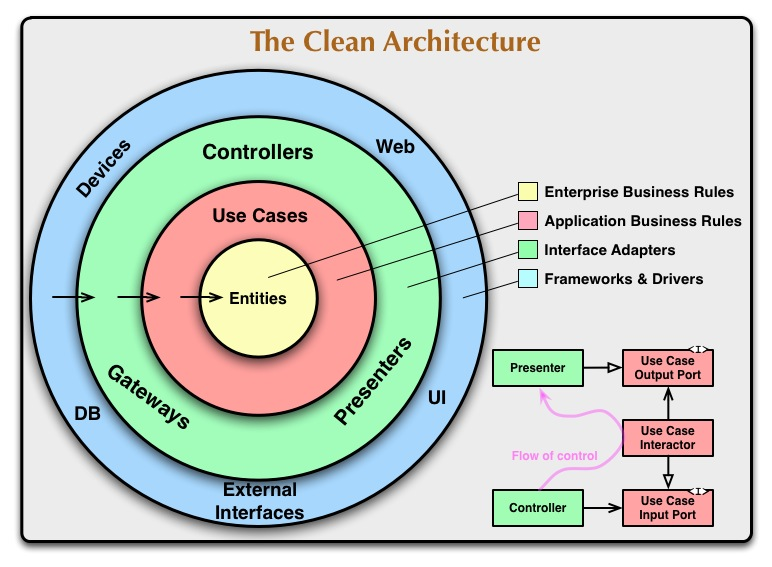
\includegraphics[width=.84\linewidth]{../images/clean-architecture-by-robert-c-martin.jpg}
    \caption{Clean architecture by Robert C. Martin \cite{unclebob2023}}\label{Fig:CABRMARTIN}
\end{figure}
\subsection{Applying Clean Architecture in Flutter}
Clean Architecture can be applied in Flutter by separating the application into three layers: Presentation, Domain, and Data. The Presentation layer handles the UI and user interactions. The Domain layer contains business logic and use cases. The Data layer manages data from various sources like network requests and databases.
\begin{figure}[H]
    \begin{minipage}{0.60\textwidth}
        \centering
        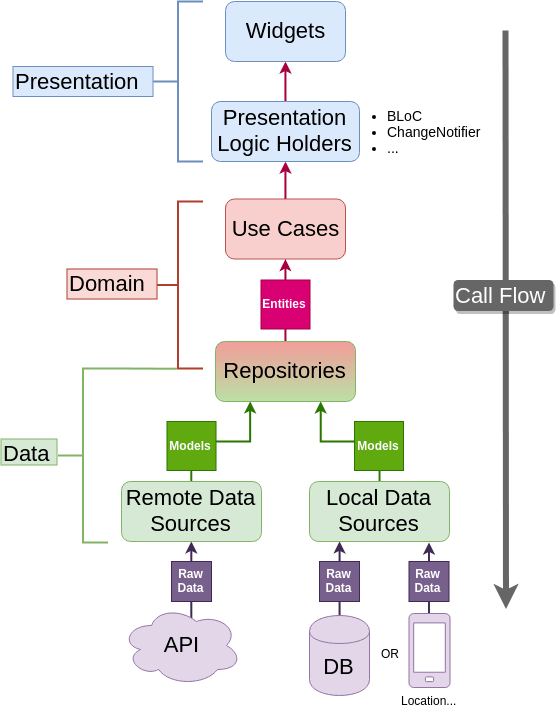
\includegraphics[width=1\linewidth]{../images/Clean-Architecture-Flutter-Diagram.png}
        \caption{Clean Architecture Diagram by Reso Coder}\label{Fig:CADRESOCODER}
    \end{minipage}\hfill
    \begin {minipage}{0.38\textwidth}
    \centering
    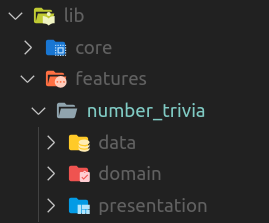
\includegraphics[width=\linewidth]{../images/number_trivia-feature-folder-structure.png}
    \caption{Example of structure in Flutter project}\label{Fig:example-flutter-ca-folder}
    \end{minipage}
\end{figure}
\section{Applications of Flutter and Clean Architecture}
\subsection{Accelerated MVP Development with Flutter}
Flutter's ability to deliver high-performance applications on Android and iOS from a single codebase makes it an excellent choice for rapid MVP development. Its rich set of widgets and reactive framework allow for a fast development cycle, enabling developers to quickly implement key features and bring the product to market.
\subsection{Case Studies of Flutter and Clean Architecture}
There are several case studies of applications developed using both Flutter and Clean Architecture. These applications demonstrate how Clean Architecture can enhance the maintainability and scalability of Flutter applications, even when under the constraints of rapid MVP development.

Flutter has been used in various real-world applications due to its ability to deliver high-performance applications on Android and iOS from a single codebase. Some examples include the Alibaba e-commerce app, the Toyota: Improving Infotainment Systems app, and Google Ads.

\begin{figure}[H]
    \begin{minipage}{0.48\textwidth}
        \centering
        
\includegraphics[width=1\linewidth]{../images/alibaba-commerce.png}
        \caption{Alibaba Group: Ecommerce}\label{Fig:AGEAPP}
    \end{minipage}\hfill
    \begin {minipage}{0.48\textwidth}
    \centering
    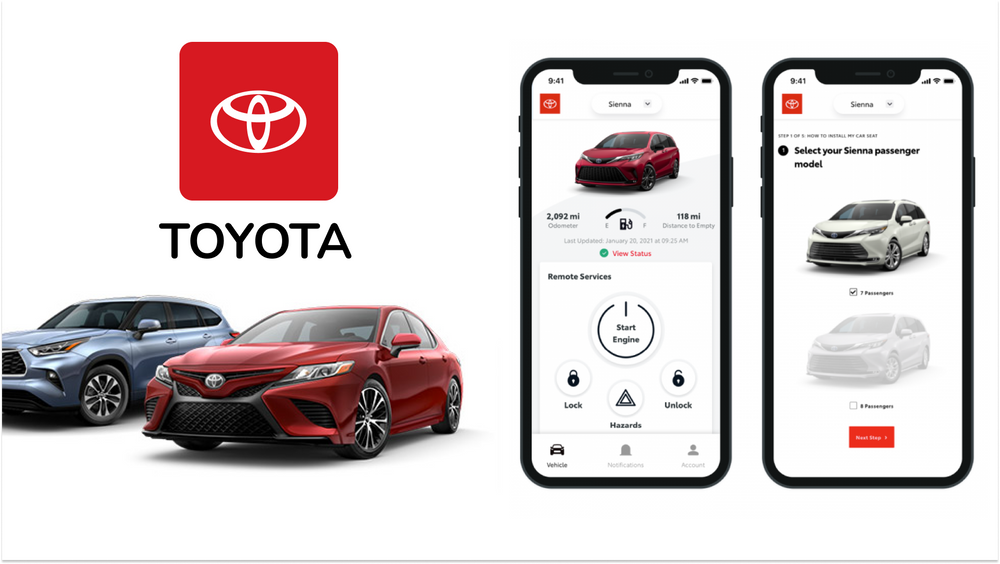
\includegraphics[width=\linewidth]{../images/TOYOTA-1.png}
    \caption{Toyota: Improving Infotainment Systems}\label{Fig:TIISAPP}
    \end{minipage}
\end{figure}
\subsection{Impact of Flutter and Clean Architecture}
The use of Flutter along with Clean Architecture has been shown to improve the development process by making it easier to manage codebases, implement new features, and fix bugs. It also enhances the performance of applications by ensuring they run smoothly on different platforms.

\section{Microservices, Flutter, and E-commerce}

\subsection{Application of Microservices and Flutter in E-commerce}
Microservices architecture and Flutter can be effectively applied in the context of e-commerce. Microservices allow for the separation of functionalities into independent services such as user authentication, product catalog, order management, and payment processing1. Flutter, with its fast development cycle and expressive UI, can be used to build the frontend of the e-commerce application.

\subsection{Benefits and Challenges}
The benefits of using these technologies in e-commerce include improved scalability, faster deployment times, better fault isolation, and more flexibility in implementing new features. However, challenges may include increased dependency on technology, large costs involved especially for small businesses, risk of job cuts due to automation, security risks related to data and fraud, and dealing with issues like shopping cart abandonment and maintaining customer loyalty.

\subsection[]{Case Studies}
Several e-commerce giants like eBay, Etsy, Gilt and Zalando have transformed their infrastructures into microservice architectures to create flexible, global systems. The combination of these technologies holds promise for efficient and scalable e-commerce application development.